\documentclass[amssymb,twocolumn,aps]{revtex4}

% allows special characters (including æøå)
\usepackage[utf8]{inputenc}
%\usepackage [norsk]{babel} %if you write norwegian
\usepackage[english]{babel}  %if you write english

\usepackage{physics,amssymb}  % mathematical symbols (physics imports amsmath)
\usepackage{graphicx}         % include graphics such as plots
\usepackage[table]{xcolor}
\usepackage{xcolor}           % set colors
\usepackage{hyperref}         % automagic cross-referencing 
\usepackage{float}			  % force placement of tables and figures

\begin{document}
	
\title{Project 1 \\
    \normalsize FYS-STK4155}
\date{\today}               
\author{Selma Beate Øvland}
\affiliation{University of Oslo}

\newpage
	
\begin{abstract}

We study polynomial regression on the noisy Runge function, comparing Ordinary Least Squares (OLS), Ridge, and Lasso. Features are standardized using only training data and the target is centered so the intercept is not penalized. Performance is evaluated with test MSE/R², and we also examine gradient-descent variants.

We find that OLS performs well at low degrees but overfits as degree increases (rising MSE). Ridge reduces error at higher degrees by shrinking coefficients; Lasso achieves comparable accuracy with sparser models and improved numerical stability. Using 10-fold cross-validation, the best OLS model is degree 8 (test MSE 0.010). For Ridge at fixed degree 10, the optimal $\lambda$ = 0.01 yields MSE 0.0094—about 22 percent lower than OLS at the same degree (0.012). Bootstrap analysis indicates Ridge slightly increases bias but more substantially lowers variance, reducing total error. Adaptive gradient methods (e.g., Adam) converge faster than fixed step sizes. Overall, cross-validation and regularization produce more robust models than plain OLS.

\end{abstract}


\maketitle

\section{Introduction}
A challenge in machine learning methods for regression is to obtain a reliable input-output relationship from data while at the same time controlling the model complexity to avoid poor generalization. While polynomials can approximate smooth functions well, high degree models are prone to numerical instability and overfitting when data is noisy or features are not properly scaled. For effective regression models we want to balance simplicity and flexibility to minimize the expected prediction error. This critical tension is summarized by the bias-variance trade-off. \cite{compfys39}. \\

A model with high bias suffers from underfitting, failing to capture the complexity of the true function. A model with high variance suffers from overfitting, meaning it has learnt the noise of the training data leading to poor generalization on unseen data \cite{compfys38}, \cite{hastie}. Our goal in this project is to explore methods that balance this trade-off, as shown in \ref{fig:biasvariance}. To obtain models that are both stable and accurate, we make use of regularization and resampling techniques. Especially for multicollinearity issues we benefit from Ridge and Lasso regression, as they introduce a penalty term to the MSE cost function forcing the model parameters towards smaller magnitude which reduce variance. \\

In the project we will use the Runge function

\begin{equation}
    f(x) = \frac{1}{1 + 25x^2}
\end{equation}

to create a synthetic dataset of evenly spaced data points. We use this function to study how fitting it with high-polynomials illustrates the issue with interpolation instability and overfitting, which is a known phenomena useful for studying regularization methods \cite{compfys}. (ref https://en.wikipedia.org/wiki/Runge%27s_phenomenon). \\
\\
We first look at fitting OLS up to degree 15 on the Runge function in part (a), where we evaluate the accuracy with MSE and $R^2$ vs degree. In part (b) we study the penalty term $\lambda$ and it's relationship to the polynomial degree again using MSE and $R^2$ analysis. In part (c-f) we replace the equations with gradient-based solvers and examine convergence under different step sizes. In part (g) we implement bootstrap to separate the error into bias and variance, to explore the effect polynomial degree and sample size will have. Part (h) implements k-fold cross-validation and compares these test errors to the bootstrap estimates. In the end, we will have a method for diagnosing underfitting and overfitting, and selecting polynomial degrees and penalty terms that work well.  


    
\section{Methods}\label{section:methods}

\subsection{Method 1/X}



\subsection{Implementation}


\subsection{Use of AI tools}
	
I used ChatGPT to help me make a plan for how to structure the code for this project. Before that, I started with part (a), wrote the code, then went to part (b) and realized I could reuse some code from part (a). I ended up with messy code without clear structure, with repeated variables and functions more times than needed. I wanted to separate the code and make it reusable for all parts of this project, and also for other projects/exercises later. So I uploaded the project description to ChatGPT and asked for a plan on how to organize the code (not the actual code). ChatGPT gave me a plan where I can make one Python file at a time (data, models, plotting, etc.), so I don’t have to think only in terms of part a, b, c, which was a bit overwhelming. This helps me keep the code cleaner and easier to reuse.
	
\section{Results and Discussion}\label{section:results} 



\begin{figure}[h]
    \centering
    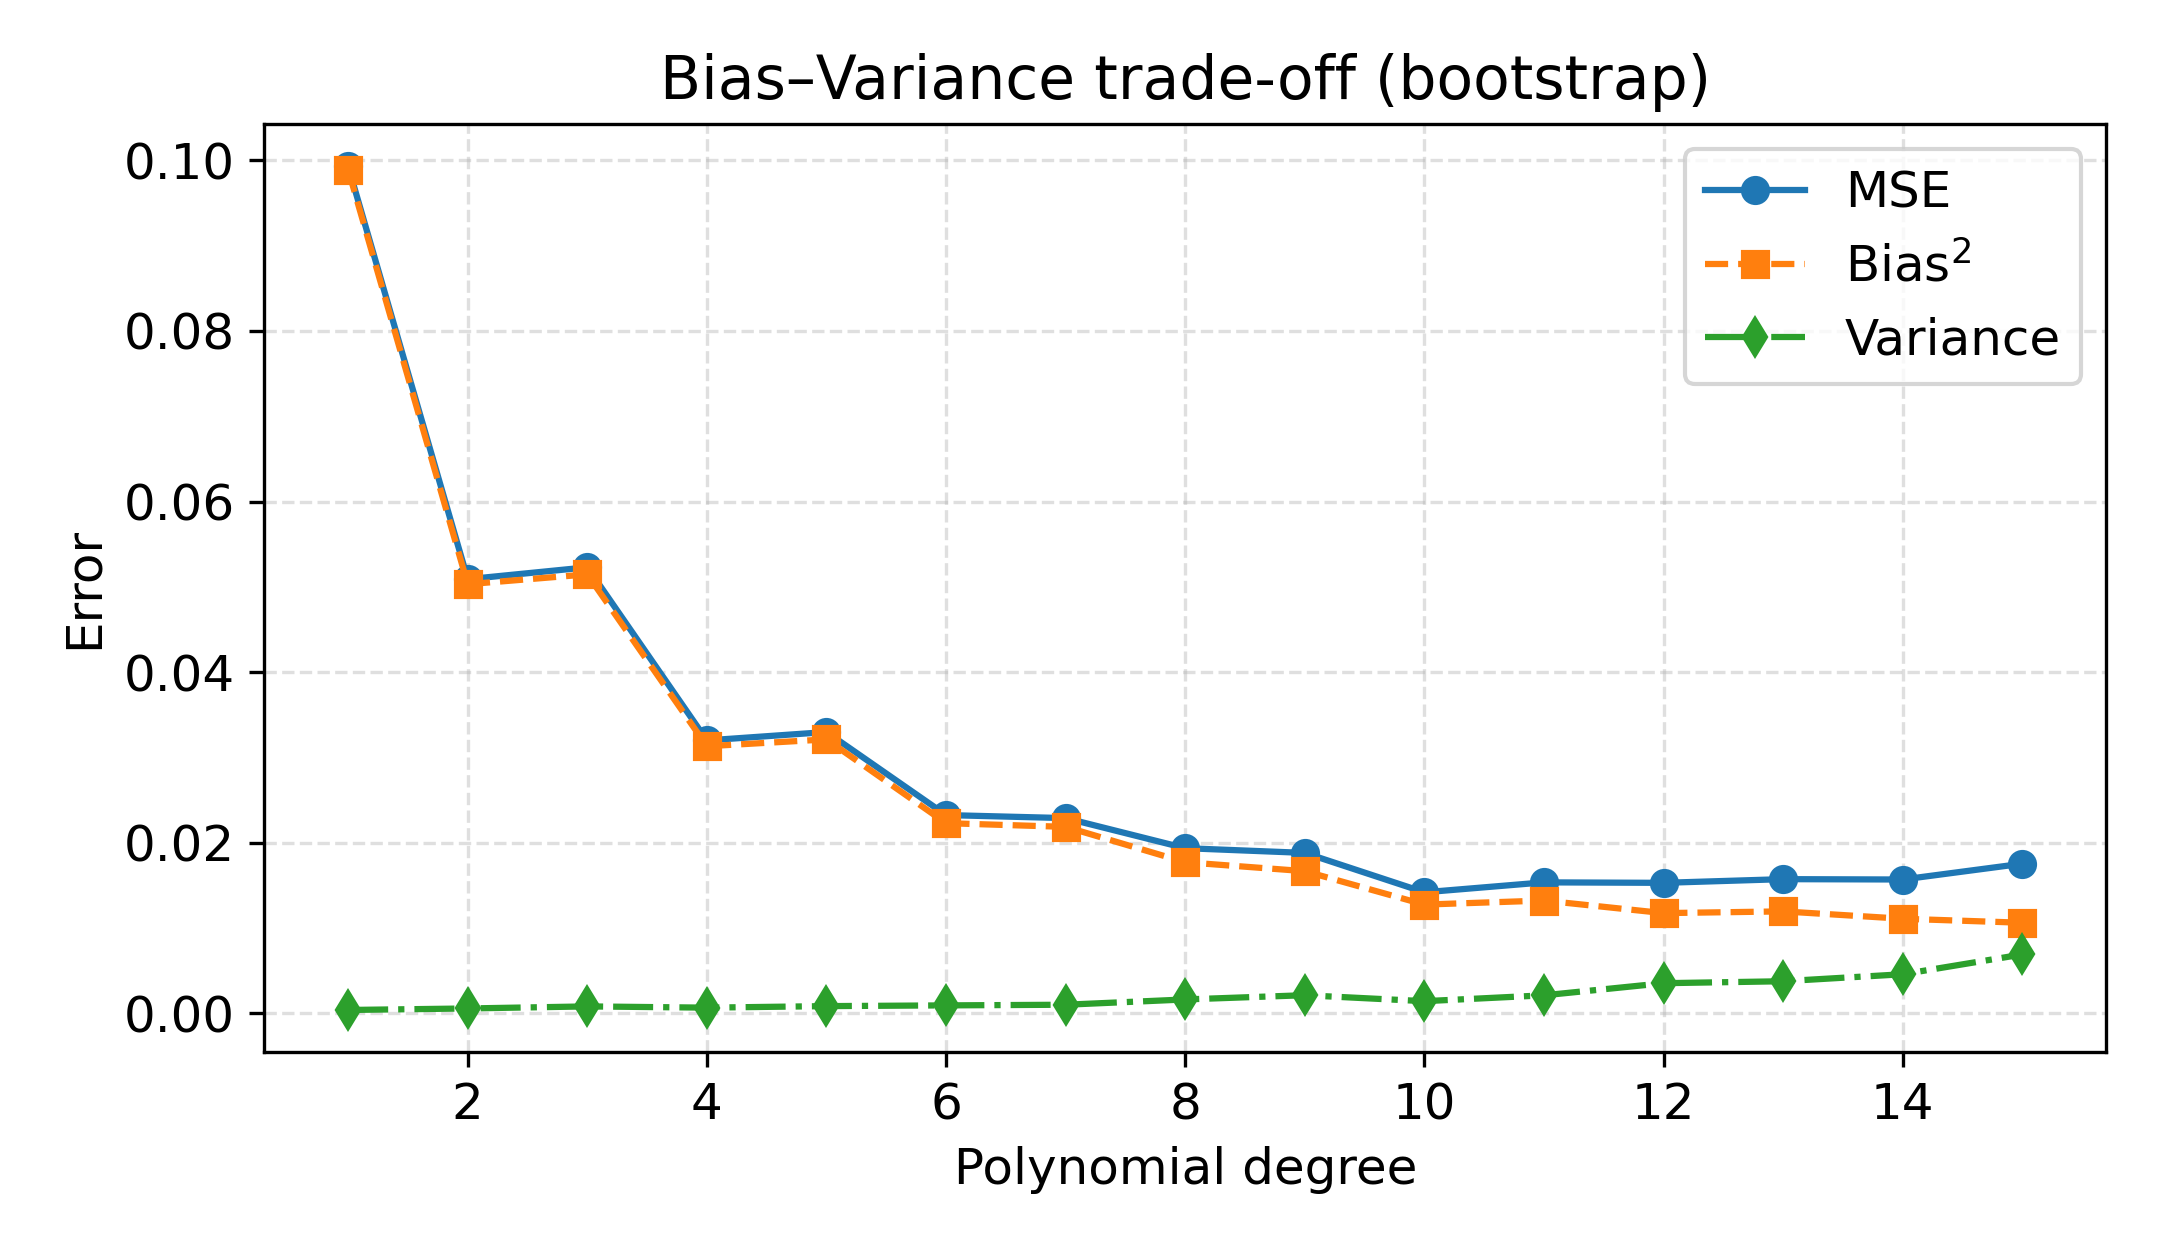
\includegraphics[width=0.5\linewidth]{Project-1/Figures/bias_variance_tradeoff.png}
    \caption{Bias–variance trade-off for polynomial regression on a noisy 1D function. For each polynomial degree on the x-axis, we see the corresponding MSE, squared bias and variance. As model complexity increases, squared bias decreases and variance increases. MSE is smallest around degree 10, in the intermediate window, showing how simpler models underfit (high bias) and complex models overfit (high variance).}
    \label{fig:biasvariance}
\end{figure}

\begin{figure}[h]
    \centering
    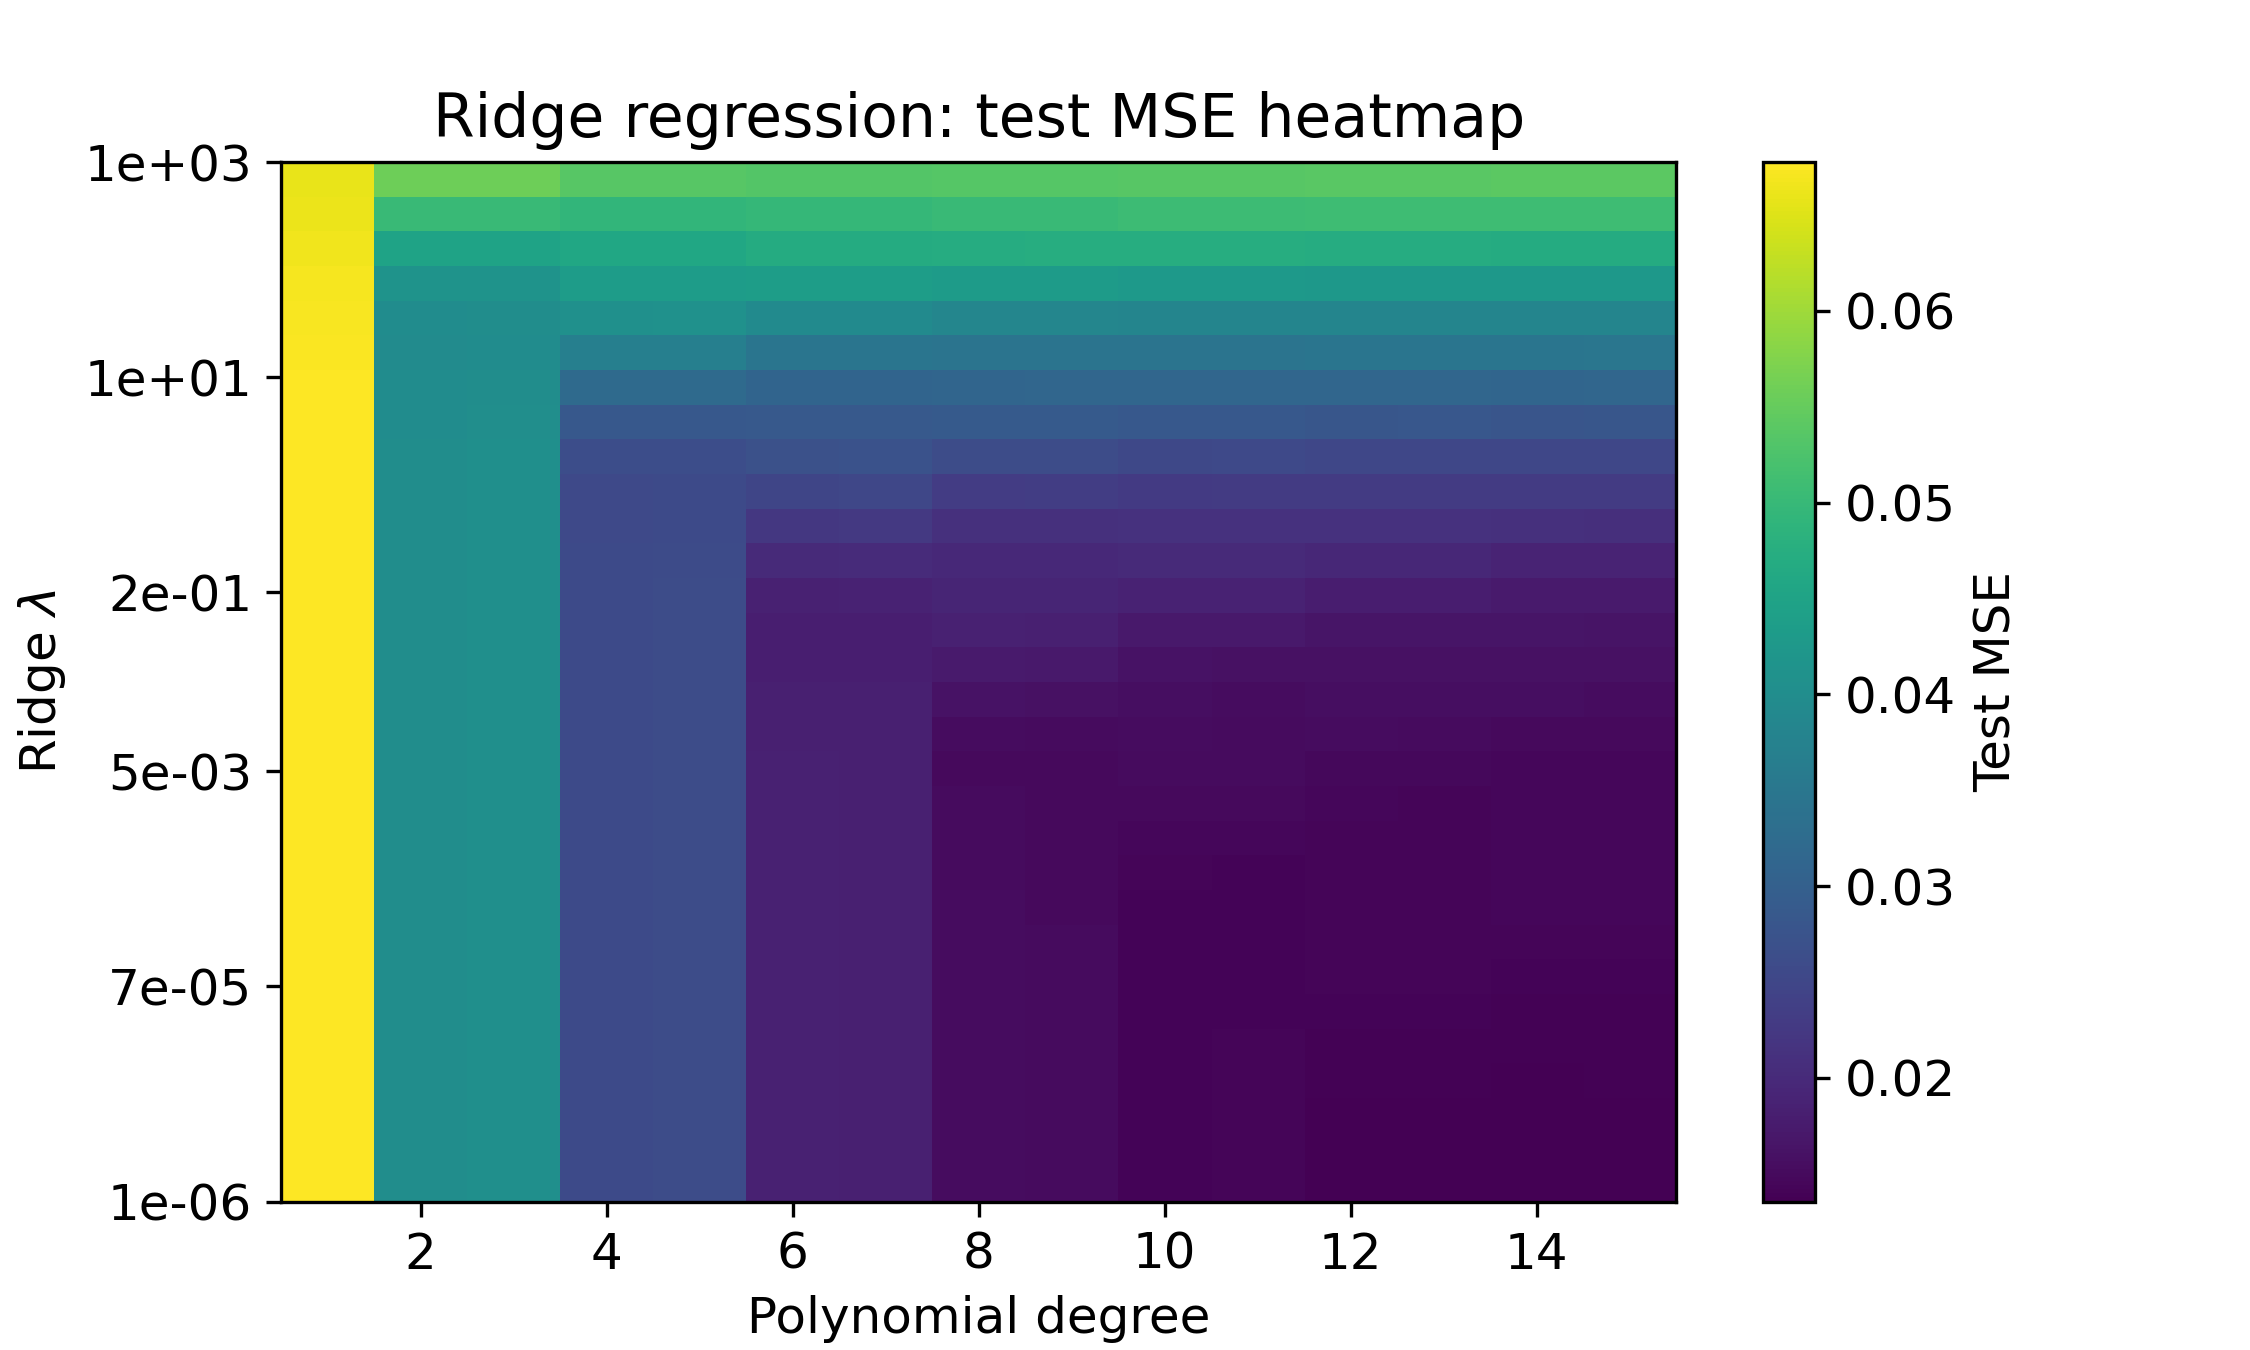
\includegraphics[width=0.5\linewidth]{Project-1/Figures/heatmap.png}
    \caption{B}
    \label{fig:biasvariance}
\end{figure}


\section{Conclusion}\label{section:conclusion} 


\bibliography{biblio}

\end{document}
